\section{Research method}

Figure \ref{fig:Research_Questions} summarizes how the questions are related and the methods used to answer them.
\begin{figure}[h]
    \centering
    \fbox{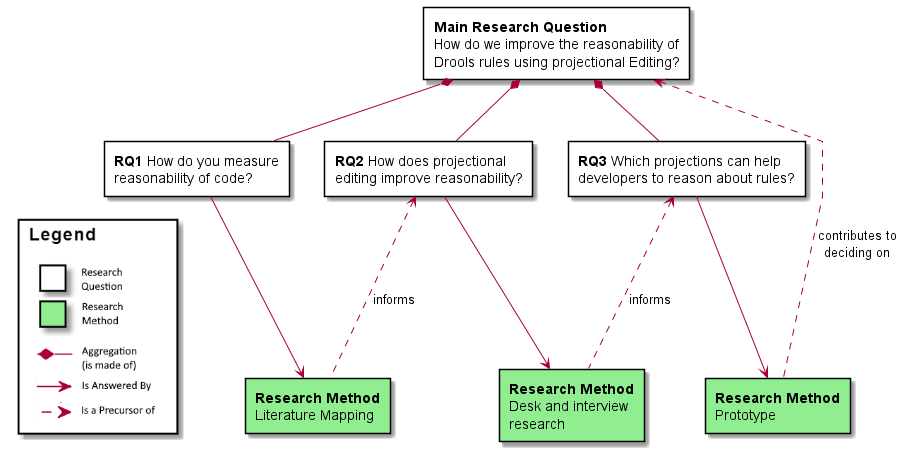
\includegraphics[width=0.95\textwidth]{images/ResearchQuestion_Legend.png}}
    \caption{Research questions and methods.}
    \label{fig:Research_Questions}
\end{figure}

As seen in figure \ref{fig:Research_Questions}, RQ 1 - ``What is the current state of language workbenches supporting projectional editing?'', will be answered by the method of conducting a literature review of the field of language workbenches, specifically regarding those that support projectional editing. 
This research method will follow the recommendations of Kitchenham et al.\cite{kitchenham2015evidence}.
To be clear on what we are investigating some terms should be defined first.
A language workbench supports the efficient development of languages. 
The term caught on after a 2005 article by Martin Fowler\cite{Fowler_lwb}. 
Editing in language workbenches has two predominant editing forms - free-form text editing and projectional editing\cite{erdweg2013state}.
Projectional editing is a method of bypassing the need for a parser and programming directly into projections of the Abstract Syntax Tree.

Gregor\cite{gregor2006nature}, gives ``A Taxonomy of Theory Types in Information Systems Research''. 
For RQ 2, ``Which projections can help developers to get appropriate feedback about rules?'', we will conduct what Gregor calls ``Type V: Theory for Design and Action''. 
The criteria for success of Type V research is that the prototype should ``include utility to a community of users, the novelty of the artefact, and the persuasiveness of claims that it is effective''.

For this project we will use the open-source language workbench Meta Programming System (MPS) from JetBrains\cite{MPS_ProductPage}.
MPS is built around the projectional editing paradigm.
There is no existing implementation of the Drools language in MPS.

Drools is nearly 20 years old and, according to awesomeopensource\cite{awesomeopensource}, it is the most appreciated opensource rules engine.
Despite this, it does not have strong IDE support.
In this project, we hope to correct this.

Thus, we will apply projectional editing techniques, through the MPS language workbench to the Drools language.
The novelty of our approach will be to create new view types specific to the needs of a Drools programmer.

We will be relying on MPS as well as other open-source components.
The reason we chose MPS is that it is the most developed of the free and open source projectional editing language workbenches\cite{erdweg2013state}.

An artefact of this master's project will be a prototype projectional editor, that will give much stronger editor support in JetBrain's IntelliJ, currently the most used Java IDE\cite{Java_usage_report}.
The prototype will consist of the Drools language, re-defined in the MPS language.  
The prototype will further consist of a set of projections of the DSL's AST.
MPS uses the Java graphics framework Swing for the creation of graphical, as opposed to textual, projections.
During the building of the prototype, we will decide upon which projections we will create. 
Some potential examples include:
\begin{itemize}[topsep=2pt,itemsep=2pt,partopsep=2pt, parsep=2pt]
    \item Visualization of order of rule execution;
    \item spreadsheet-like decision tables;
    \item or a ``group-by'' display on fact, query or function usage.
\end{itemize}

The major tasks in this prototype development will be: 
\begin{itemize}[topsep=2pt,itemsep=2pt,partopsep=2pt, parsep=2pt]
    \item Modelling the Drools language;
    \item and developing the alternative projections.
\end{itemize}

The prototype itself will be validated by working.
However, if time permits, the hypothesis of the usefulness of the projections will be further validated through developer use surveys.

